%% Draft settings
\documentclass[10pt]{article}
\usepackage{amsmath}
\usepackage{amssymb}
\usepackage{graphicx}
\usepackage{subfigure}
\usepackage{color}
 \usepackage{lineno}
\usepackage{simplemargins}
\usepackage{natbib}

% \linenumbers*[1]
 \usepackage[T1]{fontenc} % For citing barki{\dj}ija
\setkeys{Gin}{draft=false}


% Margins
\setleftmargin{1in}
\setrightmargin{1in}
\setbottommargin{1in}
\settopmargin{1in}
 
% My Commands
%\input{tensor_book_shrtcts.tex}
\newcommand{\comment}[1]{\textcolor{blue}{[{#1}]}}


%%Nadir's Shortcuts
\newcommand{\beqn}{\begin{equation}}
\newcommand{\eeqn}{\end{equation}}
\newcommand{\beqa}{\begin{eqnarray}}
\newcommand{\eeqa}{\end{eqnarray}}
\newcommand{\beqanonum}{\begin{eqnarray*}}
\newcommand{\eeqanonum}{\end{eqnarray*}}
\newcommand{\beqnonum}{\begin{equation*}}
\newcommand{\eeqnonum}{\end{equation*}}
\newcommand{\jump}{\vspace{0.5cm}}
\newcommand{\bbf}{\begin{bf}}
\newcommand{\ebf}{\end{bf}}
\newcommand{\eqnref}[1]{(\ref{#1})}
\newcommand{\defn}[1]{\begin{bf}\emph{#1}\end{bf}}
\newcommand{\reals}{\ensuremath{\mathbb{R}}}
\newcommand{\complex}{\ensuremath{\mathbb{C}}}
\newcommand{\integers}{\ensuremath{\mathbb{Z}}}
\newcommand{\half}{\ensuremath{\frac{1}{2}}}
\newcommand{\n}{\nonumber}
\newcommand{\inverse}{^{-1}}

%calculus shorthand
\newcommand{\timeder}{\frac{d}{dt}}
\newcommand{\partialder}[1]{\frac{\partial}{\partial #1}}
\newcommand{\partialderf}[2]{\ensuremath{\frac{\partial #1}{\partial #2}}}
\newcommand{\der}[2]{\ensuremath{\frac{d #1}{d #2}}}
\newcommand{\dx}{\ensuremath{\frac{d}{dx}}}
\newcommand{\ddx}{\ensuremath{\frac{d}{dx}}}
\newcommand{\kvec}{\ensuremath{\vec{k}}}
\newcommand{\uvec}{\ensuremath{\mathbf{u}}}
\newcommand{\zhat}{\ensuremath{\mathbf{\hat{z}}}}
\newcommand{\khat}{\ensuremath{\mathbf{\hat{k}}}}
\newcommand{\unitvect}[1]{\ensuremath{\mathbf{\hat{#1}}}}
\newcommand{\ppx}{\ensuremath{\partial_x}}
\newcommand{\ppy}{\ensuremath{\partial_y}}
\newcommand{\ppz}{\ensuremath{\partial_z}}
\newcommand{\ppt}{\ensuremath{\partial_T}}
\newcommand{\ppp}{\ensuremath{\partial_p}}


% radiation shorthand
\newcommand{\cotwo}{\ensuremath{\mathrm{CO_2}}}
\newcommand{\othree}{\ensuremath{\mathrm{O_3}}}
\newcommand{\htwo}{\ensuremath{\mathrm{H_2O}}}
\newcommand{\QLW}{\ensuremath{Q_\mathrm{LW}}}
\newcommand{\QSW}{\ensuremath{Q_\mathrm{SW}}}
\newcommand{\Qnet}{\ensuremath{Q_\mathrm{net}}}
\newcommand{\FLW}{\ensuremath{F^\mathrm{LW}}}
\newcommand{\FSW}{\ensuremath{F^\mathrm{SW}}}
\newcommand{\USW}{\ensuremath{U^\mathrm{SW}}}
\newcommand{\DSW}{\ensuremath{D^\mathrm{SW}}}
\newcommand{\Fnet}{\ensuremath{F^\mathrm{net}}}
\newcommand{\olr}{\ensuremath{\mathrm{OLR}}}
\newcommand{\OLR}{\ensuremath{\mathrm{OLR}}}
\newcommand{\trans}{\ensuremath{\mathcal{T}}}
\newcommand{\solar}{\ensuremath{I_0}}
\newcommand{\cool}{\ensuremath{\mathcal{C}}}
\newcommand{\cminverse}{\ensuremath{\mathrm{cm^{-1}}}}
\newcommand{\pierre}{P10}
\newcommand{\tauk}{\ensuremath{\tau_k}}
\newcommand{\Wmsq}{\ensuremath{\mathrm{W/m^2}}}

% meteorology shorthand
\newcommand{\qv}{\ensuremath{q}}
\newcommand{\rhov}{\ensuremath{\rho_\mathrm{v}}}
\newcommand{\Hv}{\ensuremath{H_\mathrm{v}}}
\newcommand{\Rv}{\ensuremath{R_\mathrm{v}}}
\newcommand{\qa}{\ensuremath{q_a}}
\newcommand{\qvstar}{\ensuremath{q^*}}
\newcommand{\Ta}{\ensuremath{T_a}}
\newcommand{\Tav}{\ensuremath{T_\mathrm{av}}}
\newcommand{\Ts}{\ensuremath{T_\mathrm{s}}}
\newcommand{\ps}{\ensuremath{p_s}}
\newcommand{\RH}{\ensuremath{\mathrm{RH}}}
\newcommand{\cld}{\ensuremath{\mathrm{Cld}}}
\newcommand{\WVP}{\ensuremath{\mathrm{WVP}}}
\newcommand{\ztop}{\ensuremath{z_\mathrm{top}}}
\newcommand{\ztp}{\ensuremath{z_\mathrm{tp}}}
\newcommand{\zlcl}{\ensuremath{z_\mathrm{LCL}}}
\newcommand{\Tlcl}{\ensuremath{T_\mathrm{LCL}}}
\newcommand{\Ttp}{\ensuremath{T_\mathrm{tp}}}
\newcommand{\ptp}{\ensuremath{p_\mathrm{tp}}}
\newcommand{\lapseav}{\ensuremath{\Gamma_\mathrm{av}}}
\newcommand{\gammaav}{\ensuremath{\Gamma_\mathrm{av}}}
\newcommand{\Kinverse}{\ensuremath{\mathrm{K^{-1}}}}
\newcommand{\Htauk}{\ensuremath{H_{\tau_k}}}

%Variables
\newcommand{\figurepath}{../figures/}


\begin{document}

%% ------------------------------------------------------------------------ %%
%
%  TITLE
%
%% ------------------------------------------------------------------------ %%


\title{Invariant Radiative Cooling and Precipitation Change}

%% ------------------------------------------------------------------------ %%
%
%  AUTHORS AND AFFILIATIONS
%
%% ------------------------------------------------------------------------ %%


 \author{Nadir Jeevanjee\footnote{Department of Physics, University of California at Berkeley, Berkeley, CA 94702  USA. jeevanje@berkeley.edu (corresponding author)} \footnote{Climate and Ecosystems Science Division, Lawrence Berkeley National Laboratory, Berkeley, CA USA} and David Romps\footnote{Department of Earth and Planetary Sciences, University of California at Berkeley, Berkeley, CA 94702  USA.} \footnote{Climate and Ecosystems Science Division, Lawrence Berkeley National Laboratory, Berkeley, CA USA}
}

\maketitle

\begin{abstract}
We show that radiative flux divergences, when considered as functions of temperature as a vertical coordinate, are insensitive to surface temperature \Ts. This \Ts-invariance  leads to simple expressions for the \Ts-dependence of column-integrated radiative cooling, and hence precipitation. In particular, these expressions allow us to predict and better understand the roughly 3\% \Kinverse\ increase in mean precipitation  found in simulations of tropical convection, without requiring any radiative transfer calculation for the perturbed state. 

%\vspace{0.5cm}
%
%
\end{abstract}


%% ------------------------------------------------------------------------ %%
%
%  TEXT
%
%% ------------------------------------------------------------------------ %%


\section {Introduction}
It is well-known that global mean precipitation increases at a rate of roughly 1-3\% \Kinverse\  in GCM warming experiments \citep{stephens2008,lambert2008,held2006}. Since condensation heating from precipitation balances atmospheric radiative cooling \citep{ogorman2012,allen2002}, one may view global mean precipitation as  fundamentally radiation-driven, and study it from that perspective. Indeed, \cite{pendergrass2014} recently explained the 1-3\% \Kinverse\ increase in precipitation through the associated increase in column-integrated radiative cooling, which (they showed) results from increased downward emission from the atmosphere at the surface, rather than an increase of upward emission at the top-of-atmosphere (TOA). What remains to be understood, however, is why this increase takes on the value that it does. Why 1-3\% \Kinverse, and not a number many times bigger, or smaller?

This paper aims  to shed some light on this question. Our approach will be complementary to that of \cite{pendergrass2014}, in that we will examine how vertically-resolved radiative cooling profiles change with warming, rather than focusing on radiative fluxes at the surface and TOA. We will spend most of our time understanding and demonstrating that these profiles behave very simply under warming, when considered as functions of temperature as a vertical coordinate. We will then use this  to make a simple estimate 
of precipitation change with warming, and will obtain numbers in the 1-3\% \Kinverse\ range, without requiring a perturbed state radiative calculation.

\section{Simulations}
Since the energetic constraint on precipitation is essentially a statement of radiative-convective equilibrium (RCE), we will study changes in precipitation in one of the simplest systems in which this constraint operates, namely tropical oceanic RCE  with fixed sea-surface temperature (SST). We simulate this system using Das Atmosph\"arische Modell \citep[DAM,][]{romps2008},   a three-dimensional, fully-compressible, non-hydrostatic cloud-resolving model, coupled to radiation via the Rapid Radiative Transfer Model 
\citep[RRTM,][]{mlawer1997}. DAM employs the six-class Lin-Lord-Krueger  microphysics scheme \citep{lin1983, lord1984, krueger1995}, and relies on implicit LES \citep{margolin2006} for sub-grid scale transport, so no explicit sub-grid scale turbulence scheme is used.
	
	Our RCE simulations ran on a square doubly-periodic domain of horizontal dimension $L=72$ km, with  a horizontal resolution of $dx=1$ km. The vertical grid stretched smoothly from 50 m resolution below 1000 m to 250 m resolution between 1000 m and 5000 m, and then to 500 m up to the model top at  30 km. We calculated surface heat and moisture fluxes using a bulk aerodynamic formula, and used a pre-industrial \cotwo\  concentration of 280 ppm with no ozone except where specified otherwise. To explore precipitation changes  with warming we ran four experiments at surface temperatures of $\Ts=(280,290,300,310)$ K. Our runs branched off the equilibrated runs described in \cite{romps2014}, and were run for 60 days  to iron out any artifacts from changing the domain and resolution. Time-mean,  domain-mean vertical profiles were derived from the last 20 days  of each run. 
	


%======================%
% Summary of Ts-invariance   %
%======================%

\section{Summary of \Ts-invariance}
The simple behavior of radiative cooling mentioned above is just that radiative flux divergences, suitably defined and  coordinatized, are independent of surface temperature \Ts\ -- in other words, they are \Ts-invariant. We summarize the physics of this here, and give the detailed argument in subsequent sections.

The root of \Ts-invariance is the key fact that  the water vapor density 
	\beqn
		\rhov =  \RH\, p_v^*(T)/R_ vT \; 
	\label{rhov}
	\eeqn
	 is (up to variations in relative humidity \RH) a function of temperature only.\footnote{Here $p_v^* = p_v^\infty \exp(-L/R_vT)$ is the vapor pressure of water ($p_v^\infty = 2.5\times 10^{11} $ Pa), and all other symbols have their usual meaning.} If we use $T$ as a vertical coordinate,  Eqn. \eqnref{rhov} then tells us that the function $\rhov(T)$ should not depend on \Ts.  We verify this by plotting $\rhov(T)$  from our RCE simulations \citep[in which \RH\ does vary, but is a function of $T$ only; cf][]{romps2014},  in Fig. \ref{rhov_fig}. Indeed, in temperature coordinates the \rhov\ profiles at different \Ts\ collapse onto a single curve, i.e. $\rhov(T)$ is \Ts-invariant.
	 
	For wavenumbers $k$ outside of spectral bands where other trace gases (like \cotwo\ and \othree) dominate, the optical depth $\tauk$ is essentially just a vertical integral of $\rhov$  times an absorption coefficient $\kappa$. The \Ts-invariance of $\rhov(T)$ then implies the \Ts-invariance of $\tauk(T)$ (see Eqn. \eqnref{tau2} and Fig. \ref{tauk} below). But the temperature at which $\tauk(T)\approx 1$  determines that wavenumber's emission to space, and thus the \Ts-invariance of \tauk\ implies a \Ts-invariance of top-of-atmosphere radiance for $k$ with $\tauk(\Ts) \gtrsim 1$. This is, of course, the familiar basis for the runaway greenhouse effect \citep[e.g.][]{goldblatt2013}.  The essence of the argument thus far goes back to \cite{simpson1928}, with further recent development by \cite{ingram2010}.
  
 To connect all this with radiative cooling, we invoke the cooling-to-space (CTS) approximation, which says that the radiative cooling \emph{at} level $T$ is just the emission to space \emph{from} level $T$ (see Appendix A for a brief review of the CTS approximation). To the degree that the CTS approximation holds, then, we should find that radiative cooling profiles, when considered as functions of $T$, are also \Ts-invariant. This is confirmed in Fig. \ref{pptflw_tinv_dam}, and serves as the basis for the simple picture of precipitation change discussed in Section \ref{sec_simple_Q}.
	
%================%
% vapor density and    %
% optical depth            %
%================%
\section{An analytic expression for \htwo\ optical depth}
	To understand and demonstrate the \Ts-invariance of \tauk\ and various flux divergences in detail,  it is useful to develop an analytical expression for \tauk\ in terms of the water vapor path \WVP. We begin with a  formula for $\tau_k$ at height $z$,  given by  Eqn. (4.67) of \cite{pierrehumbert2010}, hereafter \pierre,
	\beqn
		\tau_k = \int_z^\infty \kappa(k) \frac{p(z')}{p_0} \rhov(z') \, dz'  \; .
		\label{tau1}
	\eeqn
One may interpret \tauk\ at a given level as the ratio of the effective area of absorbers in the column above to the actual area of the column. The effective area of absorbers, at wavenumber $k$ and per unit absorber mass, is given by  the mass absorption coefficient $\kappa(k)$ ($\mathrm{m^2/kg}$), multiplied by a pressure broadening factor $p/p_0$ with reference pressure $p_0=100$ hPa. Strictly speaking, we should also include a temperature scaling factor, but we neglect this  since temperature scaling, unlike pressure broadening,  is entirely insensitive to \Ts. This omission does not affect our conclusions.  


The integral \eqnref{tau1} is evaluated approximately in Appendix \ref{appendix_tau_formula}, yielding 
	\beqn
		\tau_k(T) = \kappa(k) \underbrace{\frac{\ps}{p_0}\left(\frac{T}{\Ts}\right)^{\frac{g}{R_d\gammaav}}}_{\substack{\text{pressure} \\ \text{broadening}}} \underbrace{\WVP_0\exp\left(-\frac{L}{R_v T}\right)}_{\substack{\text{water vapor path}}} \quad 
	\label{tau2}
	\eeqn
where  $\gammaav$ is an average tropospheric lapse rate,  $\WVP_0 \equiv \RH\, p_v^\infty\, \Tav/(L\,\gammaav)$ has dimensions of WVP (i.e., $\mathrm{kg/m^2}$), $\Tav$ is an average tropospheric temperature, and \RH\ is taken constant (see Appendix \ref{appendix_tau_formula} for definition and discussion of these parameters).  Eqn. \eqnref{tau2} approximates \tauk\ as a product of a parameterized \WVP, the mass absorption coefficient $\kappa(k)$, and an approximate pressure broadening factor, and contains no unobservable, tunable parameters. The left panel of Fig. \ref{tauk} validates Eqn. \eqnref{tau2} by comparing profiles of $\tau_k$ for  $k=(100,\ 500,\ 900)\ \cminverse$, with absorption coefficient $\kappa(k)$ computed from Eqn. \eqnref{kappa_param}, where the \tauk\ profiles are computed in two ways: first,  from  Eqn. \eqnref{tau1} using \rhov\ and $p$ profiles from 300 K simulation output, and second, using Eqn. \eqnref{tau2} with the parameters \RH, \gammaav, and \Tav\ determined as  in Appendix \ref{appendix_tau_formula}.  Though biases resulting from our expression for  \WVP\ (cf. Figure \ref{wvp_check}) are certainly evident, the match between our analytical expression \eqnref{tau2} and the numerical calculation using \eqnref{tau1} is reasonable.




%The analytical expression  \eqnref{tau2} allows us to analyze the \Ts-dependence of \tauk. First, the pressure broadening factor, proportional to $p(T)$ as given by  \eqnref{pressure}, decreases as \Ts\ increases, both because of the direct dependence on \Ts\ and because \gammaav\ decreases with \Ts, at a rate of roughly $\der{\gammaav}{\Ts}= 1\times 10^{-4} \ \mathrm{m\inverse}$. Thus pressure broadening causes $\tauk(T)$ to decrease with increasing \Ts, at a rate of roughly 1.5 --  3\% \Kinverse\ (the higher rates apply in the upper troposphere where the lapse rate effect is largest). However, there is a countervailing increase of $\tauk(T)$ with \Ts\ due to the fact that $\WVP_0$ in \eqnref{tau2} depends on \gammaav, as given in \eqnref{WVP2}. This effect stems from the fixed tropopause temperature \Ttp, which means that as \gammaav\ decreases with warming, the vertical distance between a temperature $T$ and \Ttp\  (and hence the \WVP\ at $T$) are increasing. This effect brings the decrease of $\tauk(T)$ with \Ts\ down to 0 -- 2\% \Kinverse, with the largest changes still in the upper troposphere.

With the analytical expression \eqnref{tau2} for $\tauk(T)$ in hand we can now ask how this functions depends on \Ts. We expect the vertical behavior of \tauk\ to be dominated by the exponential $\exp(-L/R_vT)$, which has no \Ts-dependence. The factor of
$(T/\Ts)^{(g/R_d\gammaav)}$ coming from pressure broadening does have some \Ts-dependence, both explicitly and implicitly through \gammaav\ (which decreases with increasing \Ts), but the exponent $g/(R_d \gammaav) \approx 1/5$ so the effect is mild. There is also a mild dependence of  $\WVP_0$ on \Ts\ through \gammaav. 

We thus expect a relatively small dependence of $\tauk(T)$ on \Ts. The right panel of Fig. \ref{tauk} confirms this, showing no discernible variation in $\tauk(T)$ for $T \gtrsim 260 $ K, and at most a factor of 2 variation in $\tauk(T)$ for $T \lesssim 260$ K over our set of RCE experiments. The latter may sound substantial, but note that by \eqnref{tau2} \tauk\ varies roughly exponentially at a rate of $L/(R_vT^2) \approx  12\%\ \Kinverse$ in the upper troposphere ($T=220$ K), or a doubling every 6 K. This means that the temperature at which a given value of  \tauk\ occurs changes by at most 6 K over our range of experiments, while \Ts\ exhibits a much larger range of  30 K.


%=================================%
% Temperature invariance of flux divergence %
%=================================%
\section{Temperature Invariance of Flux Divergences}
Now that we have established the insensitivity of  \tauk\  to \Ts, we turn to the \Ts-invariance of radiative flux divergence. We will consider only all-sky flux divergences in this paper, as that is the cooling relevant to the atmospheric energy budget. Since cloud fractions in RCE are low, however (attaining a maximum of $\sim 10 \%$ at the anvil height in our simulations), it is the clear-sky physics which dominates, justifying our use of the cooling-to-space approximation below. Our argument for \Ts-invariance also likely benefits from the FAT hypothesis \citep{harrop2012,hartmann2002}, which says that anvil temperatures (and hence their downwelling emission spectra) are also \Ts-invariant. 

Though flux divergence is usually defined as a $z$-derivative of net upwelling flux, we will again find it useful to use temperature as a vertical coordinate, and so we consider the $T$-derivative of net flux. In particular, we consider the spectral longwave (LW) flux divergence at wavenumber $k$, $-\ppt \FLW_k$. This has units of $\Wmsq/\mathrm{K}/\cminverse$, and  we introduce a minus sign to maintain a consistent sign with  $\ppz \FLW_k$. The cooling-to-space approximation (Appendix \ref{appendix_cts}) says that this can be approximated as
	\beqn
		-\ppt \FLW_k \approx - \pi B_k \frac{d \trans_k}{dT}
	\label{cts_spectral}
	\eeqn
where  
	\beqn
		\trans_k\equiv \exp(-\tauk)
	\label{trans_def}
	\eeqn
	 is the transmission function,  representing the fraction of radiation emitted at a given height which travels unabsorbed out to space. For an atmospheric layer of infinitesimal depth $\Delta T$ we can interpret $-\Delta T(d\trans_k/dT)  = \Delta T (d \tauk/dT)\trans_k$ as its `emissivity to space', since $\Delta T(d \tauk/dT)$ gives the absolute  emissivity of the layer. Thus $-d\trans_k/dT$ can be thought of as an emissivity-to-space gradient, in temperature coordinates.
	 
%	  By Kirchoff's law, the emissivity of the layer from $T$ upwards is given by $1-\trans_k(T)$, and thus $-d\trans_k/dT$  is just an emissivity gradient in temperature coordinates. 
	 
	 Utilizing our expression \eqnref{tau2} for \tauk\ and integrating over wavenumbers,  we obtain the (spectrally integrated) LW flux divergence
	\beqn
		(-\ppt \FLW)(T)  = \left( \frac{g}{R_dT\gammaav} + \frac{L}{R_v T^2}\right) \int dk\, \pi B_k(T)\, \tauk(T) e^{-\tauk(T)}  \; .
	\label{cts1}
	\eeqn
The expression in parentheses in front of the integral is just $d (\ln \tauk)/dT$, i.e. an inverse  `scale temperature' for optical depth, of roughly $\mathrm{(6 -13\ K)}\inverse$. The function $\tauk \exp(-\tauk)$ in the integrand of \eqnref{cts1} has a relatively sharp peak at $\tauk=1$, reproducing the familiar rule that emission to space at a given height occurs at frequencies with roughly unit optical depth. Denote by $k_1(T)$ the wavenumber satisfying 
	\beqn
		\tau_{k_1}(T)=1 \; , 
		\n
	\eeqn
	around which such emission will be centered.  In Appendix \ref{appendix_pptf_formula} we approximate $\tauk(T)\exp(-\tauk(T))$ as a delta function centered around $k_1(T)$,  obtaining
	\beqn
		(-\ppt \FLW)(T)  = \underbrace{\pi B_{k_1}(T)}_{\substack{ \text{Planck } \\ (\mathrm{W/m^2/cm^{-1}} ) } }
					    \underbrace{\frac{1}{e}\left( \frac{g}{R_dT\gammaav} + \frac{L}{R_v T^2}\right)}_{\substack{ \text{emissivity-to-space gradient}  \\ (\mathrm{1/K}) } } 
					   \underbrace{\Delta k}_{\substack{  \text{spectral} \\ \text{width} \\ \mathrm{(cm^{-1})} } }   \; .
		\label{cts2}
	\eeqn
  The emissivity-to-space gradient is that for $k=k_1(T)$, and its relation to the optical depth scale temperature is given by 
  	\beqn
		-\left.\frac{d\trans_k}{dT}\right|_{\tauk=1}\ =\ \frac{1}{e}\frac{d(\ln\tauk)}{dT} \; ,
		\n
	\eeqn
which follows easily from \eqnref{trans_def}.  Finally, the factor $\Delta k \approx 200\ \cminverse$ is the characteristic  width of the spectral region at any given height that is actively radiating to space.  This latter agrees nicely with the spectral LW cooling plots found in, e.g., \cite{huang2013,clough1992}. The end of  Appendix \ref{appendix_pptf_formula} derives this value for $\Delta k$ from water-vapor spectroscopy. 
Note that Eqn. \eqnref{cts2} gives us a simple way of thinking about  radiative cooling (in $\Wmsq/\mathrm{K}$) at level $T$: it is just a spectral Planck emission, times a spectral width,  times an appropriate measure of emissivity. We will evaluate this expression in a back-of-the-envelope fashion in Section \ref{sec_summary}.
 
 	A numerical analysis of the factor $B_{k_1}(T)$ in \eqnref{cts2}, utilizing an inversion of \eqnref{tau2} for $k_1(T)$, shows that it decreases by at most .3\% \Kinverse\ with \Ts. The emissivity-to-space gradient  exhibits similarly small (but oppositely signed) variations with \Ts, caused by decreases in \gammaav. This suggests that variations of $(-\ppt \FLW)(T)$ with \Ts\ should be barely discernible, which we confirm in Fig.  \ref{pptflw_tinv_dam}, which plots $(-\ppt \FLW)(T)$ as diagnosed from RRTM coupled to our  RCE simulations.  That figure also plots 
$-\ppt \FLW$ as functions of $z$ and $p$, to emphasize the simplification that occurs when $T$ is used as the vertical coordinate.



A similar argument holds for the shortwave (SW) flux divergence. If $I_k$ is the incident solar flux at wavenumber $k$, and  neglecting reflection and scattering in the  near-infrared, 
%\citep[e.g.][]{frouin1990}, 
then without further approximation we have
	\beqn
		-\ppt \FSW_k = - I_k \der{\trans_k}{T}
		\
	\eeqn
\citep[c.f.][eqn. 9.26]{thomas2002}. This equation is similar to  \eqnref{cts_spectral} but with $B_k(T) \rightarrow I_k$. As a function of $k$, $I_k$ behaves very much like a translated (in $k$-space) version of  $B_k(T)$,  where $T$ is any tropospheric temperature  \citep[cf. Fig. 3.2 of][]{hartmann1994book}. Furthermore, the slopes of $\ln(\kappa(k))$ in the far-IR bands, shown in Fig. \ref{kappa_h2o}, are similar to the slopes in the near-IR bands (Fig. 5.13 of \pierre). These similarities imply that the insensitivity of $(-\ppt \FSW)(T)$ to \Ts\ should be comparable to that of  $(-\ppt \FLW)(T)$.
 This is confirmed in Fig. \ref{pptfsw_tinv_dam}, where again the simple behavior of $(-\ppt \FSW)$ in temperature coordinates is contrasted with that in height and pressure coordinates.


%=================%
% Simple picture for Q   %
%=================%
		
\section{A simple picture for column-integrated radiative cooling} \label{sec_simple_Q}
	We now employ the \Ts-invariance of radiative flux divergences  to construct a simple, quantitative picture of how column-integrated radiative cooling, and hence precipitation,  change with surface temperature. 
	
	Let $F$ denote a radiative flux in a particular channel -- LW, SW, or net (LW+SW) -- and $Q$ the associated column-integrated cooling. The basic idea is to write $Q$ as an integral of $-\ppt F$ over the free troposphere (i.e. above the lifting condensation level \Tlcl; see motivation for this below) in temperature coordinates: 
	\beqn
		Q =  \int_{\Ttp}^{\Tlcl} (-\partial_{T'} F) dT' \ . 
		\n
	\eeqn
The lower limit \Ttp\ is the tropopause temperature, defined here as the temperature at which $-\ppt F$ goes to 0. From Figs. \ref{pptflw_tinv_dam} and \ref{pptfsw_tinv_dam} we see that $\Ttp \approx 185$ K for both LW and SW channels and all \Ts, so we consider it fixed.    If we then approximate the change in LCL temperature \Tlcl\ as equal to the change in \Ts, then the change in $Q$ with surface temperature is  simply
	\beqn
		\der{Q}{\Ts} \ =\  \left.  -\ppt F\right|_{\Tlcl}  \; .
	\label{dqdts}
	\eeqn
In other words, since the tropospheric cooling profile $(-\ppt F)(T)$  is independent of \Ts, increasing \Ts\ just exposes more of this profile.  The contribution of this new section of the $(-\ppt F)(T)$ curve to $Q$ is given by \eqnref{dqdts}.  A cartoon of this argument is given in Fig. \ref{dqdts_cartoon}. For finite changes in \Ts, Eqn. \eqnref{dqdts} approximates $(-\ppt F)(T)$ in the newly exposed region as equal to $-\ppt F$ at the LCL of the base state, but for small enough changes in \Ts\ this approximation should be adequate.

Let us test the predictive power of Eqn. \eqnref{dqdts} by checking if, given output from an RCE simulation at a particular \Ts, it can predict how $Q$ will change as $\Ts$ is increased. The LCL temperature in Eqn. \eqnref{dqdts}  is diagnosed as $T$ at the low-level maximum in cloud fraction. The panels of Fig. \ref{Qnet_varsst} plot $Q(\Ts)$ as diagnosed directly from our CRM simulations, along with estimates of the slope of this curve derived using  Eqn. \eqnref{dqdts}, for the SW, LW, and net  channels. (For greater context and a more robust test of \eqnref{dqdts} we include a \Ts=320 K simulation in these plots, but postpone discussion of the $\Ts \geq 310$ K results momentarily.)  Figure \ref{Qnet_varsst} shows that, for $ 280 < \Ts < 310$ K,  equation \eqnref{dqdts} does an excellent job of capturing the changes in  cooling in all channels. Thus our observation that radiative fluxes, when considered as functions of temperature, are roughly \Ts-invariant allows us to  predict how column-integrated cooling will change, via a simple analytic formula that requires only diagnostics from the base state. In particular, the perturbed state radiative transfer calculations employed in previous studies \citep[e.g.][]{pendergrass2014,ogorman2012, held2006} are not required. 

Of course,  our interest in column-integrated radiative cooling stems from the atmospheric energy constraint on precipitation, which in its most precise form says that time and domain-mean precipitation $P$, when expressed in $\mathrm{W/m^2}$, should balance the net radiative cooling integrated over the free troposphere \citep{ogorman2012}, which is our \Qnet. We thus plot $P$ in the right panel of Fig. \ref{Qnet_varsst}, and see that for \Ts < 310 K $P$ tracks \Qnet\ closely, as expected, except for  $\Ts=280$ K, where sensible heat fluxes start to play a more prominent role.\footnote{Indeed, the sensible heat flux at \Ts=280 K  is $\mathrm{15\ W/m^2}$, which is \emph{greater} than the corresponding value of 10 \Wmsq\ for \Ts=300 K, even though the total atmospheric cooling is less than half as large.} 
 At temperatures somewhat greater than or equal to Earth's mean temperature of 288 K, though,  Eqn. \eqnref{dqdts} can indeed provide a good first-order estimate of how precipitation changes with warming, at least in our simplified RCE context. 

Let us now discuss our results for $\Ts \geq 310$ K. The simulations show a leveling off of both precipitation and \Qnet\ with \Ts, with precipitation now larger than \Qnet. Furthermore, \eqnref{dqdts} predicts (in fact, overestimates) this leveling off at \Ts=310 K, and predicts a \emph{decrease} of \Qnet\ with \Ts\ at \Ts=320 K. How should we understand these results?

Figure \ref{pptf_allchannels} shows SW, LW, and net flux divergences for all of our cases, including $\Ts=320$ K. This figure shows that the leveling off of \Qnet\ for $\Ts > 310$ K is due to $ - \ppt \Fnet$ switching sign around that temperature.  Furthermore, this change of sign is because -\ppt \FLW\ is tending towards zero with increasing $T$, while -\ppt \FSW\ is staying roughly constant. We suspect that runaway greenhouse physics, known to set in at roughly 310 K \citep{goldblatt2013}, is responsible, in that all LW wavenumbers now reach $\tauk =1$ somewhere in the atmosphere. Above this runaway temperature, then, there are no more wavenumbers left to cool to space, Eqn. \eqnref{cts2} no longer holds because there is no $k_1(T)$, and LW radiative cooling must decline. No such limit is yet reached in the SW, presumably because the minimum absorption coefficient in the SW is significantly smaller than that in the LW (Fig. 5.13 of P10), and so there are still unsaturated wavenumbers with $\tauk \ll 1 $.

Taken further, the logic above implies that there should actually be a \emph{maximum} value of \Qnet, and perhaps hence precipitation, since increasing \Ts\ will increase SW absorption -\QSW\ but not increase LW cooling \QLW. This is suggested by the negative values of -\ppt\Fnet\ for $\Ts > 310$ K, which manifests in the negative value of $d\Qnet/d\Ts$(320 K) as predicted by \eqnref{dqdts}, shown in Fig. \ref{Qnet_varsst}. Confirmation of  this in our RCE simulations is hampered, however, by the fact that for $\Ts > 320 $ K, our simulations are unstable. We speculate that this instability is related to the sign change in -\ppt\Fnet; RCE is by definition a balance between radiative cooling and convective heating, so if the radiative cooling changes to heating in the lower troposphere one might expect a fundamental shift in the nature of the system. Such a shift might also explain why $P > \Qnet$ in this regime. Note that such a relation is not impossible, but could be achieved, for instance, by an increase in the heating of the boundary layer by turbulent entrainment from the free troposphere.

Finally, we note that even though our theory qualitatively captures this decline in \Qnet\ near the runaway regime, its quantitative accuracy starts to degrade. This is due to the fact that \Ts-invariance is only an approximation, and there is some spread between $-\ppt \Fnet$ profiles for different \Ts, as visible in Fig. \ref{pptf_allchannels}. This spread is greatest around 275 K, close to the stable layer caused by the melting line, as well as to the temperatures where \htwo\ lines in the 660 \cminverse \cotwo\ band would be cooling to space, were it not for the presence of \cotwo\ \citep[cf. Fig. 1 of][]{huang2013}.  The change in stability around the melting line likely causes some radiative heating through the exchange terms \eqnref{exch_below} and \eqnref{exch_above}, which the CTS approximation neglects, and the effects of \cotwo\ are not included in our expression \eqnref{cts2}. Thus, one might expect that eliminating these effects would yield a greater \Ts-invariance in $-\ppt \FLW$ and $-\ppt \Fnet$. We tested this by running  simulations without fusion\footnote{This is done by setting the difference in heat capacities, as well as the energy difference between liquid and solid water at the freezing point, to zero. This is similar to the `without ice' runs of \cite{seeley2016}, except that we do not alter the radiation scheme, nor do we homogenize fall speeds across hydrometeor species.} or \cotwo, and indeed found that this largely eliminated the spread.


%===========%
% Discussion    %		
%===========%

\section{Summary and discussion} \label{sec_summary}
Our results can be summarized as follows:
\begin{itemize}
	\item The manifest \Ts-invariance of \rhov\ as a function of temperature (cf. Eqn. \eqnref{rhov} and Fig. \ref{rhov_fig}) leads to a \Ts-invariance of optical depth, as seen in Fig. \ref{tauk}.
	\item This, combined with the cooling-to-space approximation, suggests that SW and LW flux divergences should also be \Ts-invariant functions of temperature, as confirmed in Figs. \ref{pptflw_tinv_dam} and \ref{pptfsw_tinv_dam}.
	\item This \Ts-invariance of flux divergences leads to a simple formula, Eqn. \eqnref{dqdts}, for how column-integrated radiative cooling increases with \Ts. This formula is validated in Fig. \ref{Qnet_varsst},  and requires no perturbed state radiative transfer calculation.
	\end{itemize}

As mentioned in the introduction, the major motivation for this work was to better understand the 1-3\% \Kinverse\ increase in global mean precipitation found in GCM warming experiments \citep{stephens2008, lambert2008,held2006}.  Our results imply that the fractional change in precipitation from warming can be estimated as 
	\beqn
		\frac{d \ln  P}{d \Ts} \ \approx\  \frac{(-\ppt \Fnet)(\Tlcl)}{\Qnet} \; .
	\label{precip_estimate}
	\eeqn
For \Ts=300 K, where $(-\ppt \Fnet)(\Tlcl) \approx 3 \ \Wmsq/\mathrm{K}$ and $\Qnet\ =\  104\ \Wmsq$, this  gives  3\% \Kinverse. Combining this with an estimated -1 \Wmsq/K from direct CO2 forcing \citep{pendergrass2014}, we obtain a net fractional increase of 2\% \Kinverse\ for energetically consistent warming, in good agreement with GCM results.

Of course, Eqn. \eqnref{precip_estimate}  just pushes the question back to what determines $\Qnet$ and $\ppt \Fnet$.  While a complete answer must await further work, we note that the approximate expression  \eqnref{cts2} for $-\ppt \FLW$ allows for a back-of-the-envelope calculation for LW cooling, as follows.   Taking $T=270$ K, which corresponds to a $k_1(T)$ of 500 \cminverse, we find $\pi B_{k_1}(T) \approx 0.35 \ \Wmsq/\cminverse$. The `scale temperature' $(d \ln \tauk/d T)\inverse$ at 270 K is roughly 10 K, and $\Delta k \approx 200 \ \cminverse$. Putting this all together yields $(-\ppt \FLW)(270\ \mathrm{K}) \approx 2.5 \ \Wmsq/\mathrm{K}$, reasonably close to the RRTM-diagnosed values shown in Fig. \ref{pptflw_tinv_dam}. Note that this is almost a first-principles estimate: the only empirical ingredient is our parameterization of water-vapor spectroscopy in Eqn. \eqnref{kappa_param}, which was used to estimate $\Delta k$.

A more empirical but potentially more intuitive way to understand the $\mathcal{O}(1 \%\ \Kinverse)$ increase in \Qnet\ is to note that $\ppt \Fnet$ is $\mathcal{O}(1\ \Wmsq/\mathrm{K})$ throughout virtually all of the troposphere. Thus its integral $\Qnet =  \int_{\Ttp}^{\Tlcl} (-\partial_{T'} \Fnet) dT'$  should be roughly proportional to the tropospheric depth in temperature coordinates, $\Tlcl - \Ttp \approx 100$ K.  A 1 K increase in \Ts\ (and hence \Tlcl) is a $1\%$ increase in tropospheric depth, and thus tropospheric depth and hence \Qnet\  increase at  $\mathcal{O}(1 \%\ \Kinverse)$.

While these results do give us some additional understanding of how \Qnet\ increases with warming, how can we square them with the insight of \cite{pendergrass2014} that the increase in \Qnet\ stems from an increase in LW downwelling surface radiation (DSR)? Just as OLR at a given wavenumber originates from unit optical depth below TOA, DSR at a given $k$ originates from unit optical depth above the surface. Thus, optically thin $k$ that do not experience $\tauk \approx 1$ anywhere in the atmosphere cannot contribute to either the OLR or the DSR. 
 Now, Eqn. \eqnref{cts2} says that when surface warming creates a layer of atmosphere with new temperature $T'$,  the cooling from that layer occurs at a wavenumber $k_1(T')$ which was previously optically thin but now satisfies $\tau_{k_1(T')} = 1$. Thus this wavenumber can now both cool to space \emph{as well as} contribute to the downwelling LW at the surface. Thus, additional cooling-to-space goes hand-in-hand with additional DSR, consonant with the view of \cite{pendergrass2014}.

An obvious next question about our results is to what extent they hold in climate regimes other than RCE.  Are radiative  flux divergence profiles (in temperature coordinates) the same the world over, regardless of season or latitude? On the one hand,  our argument ultimately rests on the inviolable exponential dependence of water vapor on temperature \eqnref{rhov} and fundamental principles of radiative transfer, neither of which should vary over space or time. On the other hand,  the universality of the $(-\ppt F)(T)$ profiles shown in Figs. \ref{pptflw_tinv_dam} and \ref{pptfsw_tinv_dam}  may result from the fact that \RH\ is a function of $T$ in RCE \citep{romps2014}, and that cloud fraction in our RCE runs is low, so that our clear-sky argument applies. Large variations in \RH\ or cloud-radiative effect between different climate regimes could cause significant variations in  $(-\ppt F)(T)$. Future work will investigate this.

Another question raised by our results is the nature of RCE in the `post-runaway' regime of $\Ts \gtrsim 310 $ K. A detailed analysis of the boundary-layer and free tropospheric energy balance would help us understand if RCE fundamentally changes in this regime.


%Even if there is no single, universal  $(-\ppt F)(T)$ profile for the whole globe, if $\ppt F(T)$ \emph{is} invariant for individual columns under warming, as found here for RCE, then we can estimate $dQ/d\Ts$ for that column using \eqnref{dqdts}. Using the spatial pattern of warming predicted by GCMs \citep[see, for example, Fig. 12.10 of][]{collins2013}, one could then weight the column values of $dQ/d\Ts$ by the expected warming of that column for a $1^\circ$ global mean warming, and thus obtain a robust, observationally-based estimate for global precipitation change that only relies on relatively robust model-predicted warming, rather than on relatively uncertain model-predicted changes in the hydrological cycle \citep{fildier2015,deangelis2015}.

More broadly, our results, along with other recent discoveries such as the fixed $\RH(T)$ curve of \cite{romps2014} and the Fixed Anvil Temperature of \cite{hartmann2002}, suggest that the atmosphere sometimes looks simpler when temperature is used as a vertical coordinate.  In contrast, feedback analyses typically use pressure as a vertical coordinate, and fields such as cloud fraction (denoted \cld) are considered to have `changed' between control and perturbed state simulations when their profiles as a function of $p$ have changed. In such a framework, high anvil clouds with fixed temperatures and hence fixed thermal emission to space constitute a positive feedback, because the `reference response' \citep{held2012} holds $\cld(p)$ fixed  while the atmosphere warms, artificially warming the anvils. When $\cld(p)$ is allowed to change, the anvils  return to their natural temperature, but this is regarded as a cooling of the anvils, and thus the ensuing LW cloud feedback is positive. This artificial anvil cooling exists only relative to the reference response, which conventionally uses pressure coordinates; a switch to $T$ coordinates would eliminate this.

%The use of temperature coordinates for feedback analyses was also advocated for by \cite{ingram2010}.  That paper, along with the study of \cite{simpson1928} which inspired it, prefigure many of the results given here. who also demonstrated the \Ts-invariance of optical depth profiles.  

Finally, we should re-emphasize that many elements of this work have appeared in the literature before. The \Ts-invariance of cooling-to-space profiles in temperature coordinates dates back almost one hundred years to \cite{simpson1928}, who explored its implications in a gray context. That this invariance results from the \Ts-invariance of optical depth profiles was pointed out by \cite{ingram2010}. Our main contribution here has been to further formalize this invariance, using a spectrally-resolved framework, and to then apply it to atmospheric radiative cooling, rather than OLR \citep{simpson1928} or the water-vapor feedback \citep{ingram2010}. 


%===========%
% Appendix       %		
%===========%

\section*{Appendix}

	%==================%
	% appendix_tau_formula  %
	%===================%


\appendix
	

	\section{Analytic formula for optical depth}	 \label{appendix_tau_formula}	
To make the expression   \eqnref{tau1}  analytically tractable, we make several simplifications.  First, since the integral in \eqnref{tau1} is dominated by values of the integrand close to $z$, we evaluate $p$  at $z$ and pull it out of the integral. This allows us to write $\tau_k$ in terms of the water vapor path $\WVP\equiv \int_z^\infty  \rho_v\, dz'$ as
	\beqn
		\tau_k =  \kappa(k) \frac{p}{p_0} \cdot \WVP \; .
	\label{tauWVP}
	\eeqn
To estimate the water vapor path, we also view \WVP\ as a function of temperature only, and using \eqnref{rhov} write it as 
	\beqn
		\WVP(T) =\frac{ \RH\, p_v^\infty}{R_v \gammaav}\int^T_{\Ttp} \frac{e^{-L/R_v T'}}{T'}\; dT' \; 
	\label{WVP1}
	\eeqn	
where we assume a constant, average lapse rate $\gammaav$, and we take the lower limit of our integral to be the tropopause temperature $\Ttp\approx 185$ K, where both LW and SW cooling go to 0 (Figs. \ref{pptflw_tinv_dam} and \ref{pptfsw_tinv_dam}). This neglect of stratospheric water vapor does not affect our results. 

	To evaluate the integral in \eqnref{WVP1}, we switch variables to $x\equiv L/R_v T$, which gives
	\beqn
		\int^T_{\Ttp} \frac{e^{-L/R_v T'}}{T'}\; dT' \ = \ \int_x^{x_\mathrm{tp}} \frac{e^{-x'}}{x'} dx' \ \approx\ \frac{1}{x_{\mathrm{av}}}\int_x^{x_\mathrm{tp}} e^{-x'} dx' \ \approx\ \frac{e^{-x}}{x_{\mathrm{av}}}.
		\label{int_approx}
	\eeqn
To make the first approximation above we note that $x'$ varies between 18 and 29 as $T'$ varies between $300$ K and $\Ttp$, and so the exponential $e^{-x'}$ is varying much more than the factor of $1/x'$. We thus set the latter  to $1/x_{\mathrm{av}}\equiv R_v \Tav/L$ where $\Tav \equiv (\Ts + \Ttp)/2$ and \Ts\ is the surface temperature, and pull $1/x_{\mathrm{av}}$ outside the integral. The last approximation follows from neglecting the boundary term $e^{-x_\mathrm{tp}}$. Plugging \eqnref{int_approx} into \eqnref{WVP1} then yields 		\beqn
		\WVP(T) =\WVP_0\exp\left(-\frac{L}{R_vT}\right),\quad \mbox{where}\quad  \WVP_0 \equiv \frac{\RH\, p_v^\infty\, \Tav}{L\,\gammaav} \; .
	\label{WVP2}
	\eeqn
(The quantity $\WVP_0$ should be interpreted as a characteristic, though not necessarily realistic, value of \WVP, analogous to $p_v^\infty$ for $p_v^*$.)  As a  check, Figure \ref{wvp_check} juxtaposes \WVP\ diagnosed from a CRM RCE simulation with \Ts=300 K with \WVP\ estimated via \eqnref{WVP2}, with \RH\ set to 70\% for the latter by eyeball fit and \gammaav\ diagnosed via \eqnref{gamma_diag} below. The constant \RH\ assumption underestimates boundary layer \WVP, and neglect of the ice phase (and concomitant lower saturation vapor pressure) leads to a slight overestimate of WVP at upper levels, but otherwise the fit is decent.

 We can now  plug \eqnref{WVP2} into \eqnref{tauWVP}, but  since \WVP\ is naturally a function of temperature, we should express $\tau_k$ as a function of temperature as well. This means writing $p$ as 
	\beqn
		p=\ps(T/\Ts)^{g/(R_d\gammaav)} \; ,
	\label{pressure}
	\eeqn 
	which is the expression for $p(T)$ for an atmosphere with constant lapse rate $\gammaav$. We diagnose \gammaav\ for a given simulation by evaluating \eqnref{pressure} at \Ttp\ and solving for  \gammaav, i.e.
	\beqn
		\gammaav = \frac{g}{R_d}\frac{\ln (\Ttp/\Ts)}{\ln(\ptp/\ps)}
	\label{gamma_diag}
	\eeqn
	where \ptp\ is the pressure at $T=\Ttp$. Putting all this together finally yields our  analytical expression for $\tau_k$ in terms of elementary functions,
	\beqn
		\tau_k(T) = \kappa(k)\,  \frac{\ps}{p_0}\left(\frac{T}{\Ts}\right)^{\frac{g}{R_d\gammaav}}\cdot \WVP_0\exp\left(-\frac{L}{R_v T}\right) \quad ,
	\n
	\eeqn
which is just Eqn. \eqnref{tau2}. 


	%==================%
	% appendix_pptf_formula  %
	%===================%

	\section{Spectral integral of $-\ppt F_k$} \label{appendix_pptf_formula}
	To evaluate the spectral integral in \eqnref{cts1}, we first restrict the integral to the  $(0,1000\ \cminverse)$ water vapor rotational band in which most radiative cooling occurs.  Fig. 4.19 of \pierre, reproduced in Fig. \ref{kappa_h2o}, shows that the median absorption coefficient $\kappa(k)$ in this band (as computed in sub-bands of width 50 \cminverse) can be roughly parameterized as 
		\beqn
			\kappa(k) \approx \kappa_0 \exp(-k/l_k), 
		\label{kappa_param}
		\eeqn
		where $\kappa_0 = 50\ \mathrm{m^2/kg}$ and $l_k \approx 65\ \cminverse$. The `scale wavenumber' $l_k$  exerts a strong influence  on the magnitude of LW flux divergence, as we'll see. Now,  for the tropospheric temperatures we consider, the spectral range of $\tauk(T)$ is essentially $(0,\infty)$, and in particular always includes \tauk=1. Let us denote the wavenumber at this peak as $k_1(T)$, i.e.  $\tau_{k_1(T)}=1$.  Since the function $\tauk \exp(-\tauk)$ has an integral of 1 across $(0,\infty)$ with a peak  at $\tauk=1$,  we  approximate it as a Dirac delta function $\delta(\tauk- 1)$. Transforming to $k$-coordinates then yields
       \begin{align}
                \tau_k e^{-\tau_k} & \approx \delta(\tau_k- 1)  \n \\
                                            & = \left|\partialderf{\tau_k}{k}(k_1)\right|\inverse\delta(k-k_1) \n  \\
                                            & =  \left|\partialderf{\ln\tau_k}{k}(k_1)\right|\inverse\delta(k-k_1) \n  \\ 
                                            & =  \left|\der{\ln\kappa}{k}(k_1)\right|\inverse\delta(k-k_1) \n \\
                                            & = l_k\,  \delta(k-k_1) \n \label{delta_approx}
        \end{align}
where the first equality is the standard chain rule for the delta function, the second equality follows from $\tau_{k_1}(T)=1$, the third from \eqnref{tau2}, and the fourth from \eqnref{kappa_param}. Plugging this into \eqnref{cts1}, evaluating the (now trivial) integral, and making the identification 
	\beqn
		\Delta k/e = l_k
		\n
		\label{Deltak}
	\eeqn
	then yields Eqn. \eqnref{cts2}. We introduce the factor of $1/e$ so that we may properly identify the emissivity-to-space gradient in Eqn. \eqnref{cts2}. Note that $l_k$ sets the width $\Delta k$ of the spectral region at a given height that exhibits significant cooling to space. The constancy of  $l_k$ implies the constancy of  $\Delta k$, as seen in, e.g., Fig. 1 of \cite{huang2013}.


	%============%
	% appendix_cts  %
	%===========%

	\section{The cooling-to-space approximation} \label{appendix_cts}
For completeness, this appendix briefly reviews the cooling-to-space approximation, deriving Eqn. \eqnref{cts_spectral}. A textbook treatment may be found in, e.g., \cite{thomas2002}.

Consider a single longwave frequency $k$, with optical depth profile $\tauk(z)$ (we'll work here in conventional $z$ coordinates). The fraction of radiation emitted from height $z_1$ which survives unabsorbed up to height $z_2$ is given by the generalized transmission function
	\beqn
		\trans_k(z_1,z_2)\  \equiv\ \exp\{-[\tauk(z_1) -\tauk(z_2)]\} \; .
		\n
	\eeqn
Setting $z_2=\infty$ gives the transmission function \eqnref{trans_def}.

One can then write the upwelling and downwelling fluxes $U_k(z)$ and $D_k(z)$ at wavenumber $k$ as (\pierre)
	\begin{align}
		U_k(z) & =\ U_k(0)\,\trans_k(0,z) + \int_0^z \pi B_k(z') \der{\trans_k(z',z)}{z'}dz' \n \\
		D_k(z) & =\ - \int_z^\infty \pi B_k(z') \der{\trans_k(z,z')}{z'}dz' \; . \n
	\end{align}

Differentiating these expressions  then yields an expression for the spectral flux divergence $\ppz (U_k-D_k)$ :
	\beqn
		\ppz(U_k-D_k)(z) \ = \  U_k(0) \der{\trans_k(0,z)}{z}  - 2 \pi B_k(z)\der{\tauk}{z}
									+  \int_0^z\pi B_k(z')\frac{\partial^2 \trans_k(z',z)}{\partial z' \partial z}dz' 
									+ \int_z^\infty\pi B_k(z')\frac{\partial^2 \trans_k(z,z')}{\partial z\partial z'}dz' \; .
		\n
	\eeqn
The key step is to now replace $B_k(z')$ with $[B_k(z')-B_k(z)]+B_k(z)$ in each of the last two terms. Rearrangement, as well as integration of total derivatives and some subsequent cancellation, yields
	\begin{subequations}
	\begin{align}
			\ppz(U_k-D_k)(z) \ =\  & \ \   [U_k(0)-\pi B_k(z)]\der{\trans_k(0,z)}{z} 
											& & \text{Surface exchange}  \label{exch_surf} \\
								& +\ \pi B_k(z)\der{\trans_k(z,\infty)}{z} 
											& & \text{Cooling-to-space} \label{cts_term} \\
								& +\ \int_0^z \pi [B_k(z')-B_k(z)]\frac{\partial^2\trans_k(z',z)}{\partial z' \partial z}dz' 
											& &\text{Exchange below}  \label{exch_below}  \\
								& +\  \int_z^\infty \pi [B_k(z')-B_k(z)]\frac{\partial^2\trans_k(z,z')}{\partial z \partial z'}dz' 
											& &\text{Exchange above} \; .  \label{exch_above} 
		\end{align}
		\label{cts_full}
	\end{subequations}
	The second derivatives $\frac{\partial^2\trans_k}{\partial z\partial z'} =  \frac{d \tauk}{dz}(z)\frac{d \tauk}{dz'}(z')\trans_k(z,z')$ are just the product of differential emissivities for the layers at $z$ and $z'$, times the transmission function between the layers. Multiplied by $dz'$ and  $\pi [B_k(z')-B_k(z)]$, they give the cooling (in $\mathrm{W/m^3/\cminverse}$) at height $z$ by radiative exchange  between that height and a layer of thickness $dz'$ at height $z'$. Integrating over $z' < z$ and $ z' >z$ then gives the exchange terms 
\eqnref{exch_below} and \eqnref{exch_above}.
	
	The cooling-to-space (CTS) approximation consists of neglecting these exchange terms, since it is observed  in practice that they are comparable in magnitude but opposite in sign (due to heating from below and cooling from above). The surface exchange term  \eqnref{exch_surf} is also neglected. With these approximations, and a change to $T$ as the independent variable, \eqnref{cts_full} reduces to \eqnref{cts_spectral}.
	
	We are not aware of any rigorous justification for the CTS approximation. Previous studies have, however, checked the approximation numerically in various cases,  and have found good qualitative agreement. Furthermore,  quantitative errors in vertically resolved cooling rates from the CTS approximation are typically  25\% or less  \citep{clough1992, fels1975,rodgers1966}.  As a quick, gross estimation of how good the CTS approximation is, we note that CTS term \eqnref{cts_term} gives the exact contribution from height $z$ to the TOA radiance at wavenumber $k$. If now integrate over height and wavenumber space, we see that the CTS approximation says that the column-integrated longwave radiative cooling (including the boundary-layer contribution)  should equal  the atmospheric contribution to the outgoing longwave radiation (OLR) at  TOA. The surface contribution can be bracketed by the deep tropical all-sky and clear-sky values of $\sim 20 \ \Wmsq$ and $\sim 40\ \Wmsq$ from \cite{costa2012}.   For our $\Ts=300$ K simulation, the column-integrated longwave radiative cooling (as diagnosed from RRTM) is $194\ \Wmsq$. The OLR (diagnosed via RRTM) minus the surface contribution (as estimated above) is 213--233 \Wmsq , yielding an error in the column and spectrally integrated CTS approximation of 10--20\%.


	
%========%
% Figures    %
%========%
\pagebreak

%Figure rhov_fig
\begin{figure}[h]
	\begin{center}
			\includegraphics[scale=0.7]{../figures/rhov.pdf}
		\caption{Profiles of \rhov\ from our RCE simulations at various SST, plotted using temperature as a vertical coordinate and with both linear and log scales. When plotted this way, the \rhov\ profiles at different \Ts\ collapse onto a single curve, i.e. $\rhov(T)$ has no \Ts\ dependence. 
		\label{rhov_fig}
		}
	\end{center}
\end{figure}


%Figure tauk
\begin{figure}[h]
	\begin{center}
			\includegraphics[scale=0.7]{../figures/tauk.pdf}
		\caption{\textbf{Left}: Profiles of $\tau_k(T)$ for $k=$ 100, 500, and 900 \cminverse\ as diagnosed from \eqnref{tau1} (solid) and \eqnref{tau2} (dashed), respectively. \textbf{Right}: Profiles of $\tau_k(T)$ from \eqnref{tau2} for $k=$ 100, 500, and 900 \cminverse\ and for \Ts=(280,\ 290,\ 300,\ 310) K (cold to warm colors).
		\label{tauk}
		}
	\end{center}
\end{figure}


%Figure pptflw_tinv_dam
\begin{figure}[h]
	\begin{center}
			\includegraphics[scale=0.6]{../figures/pptflw_tinv_dam.pdf}
		\caption{LW flux divergence  $-\ppt F$, as diagnosed from RRTM coupled to our CRM RCE simulations at \Ts=(280,\ 290,\ 300,\ 310) K. Fluxes are plotted from the lifting condensation level of each simulation to 22.5 km for clarity, and  in height, pressure, and temperature coordinates to emphasize the \Ts-invariance of  $(-\ppt F)(T)$.
		\label{pptflw_tinv_dam}
		}
	\end{center}
\end{figure}

%Figure pptfsw_tinv_dam
\begin{figure}[h]
	\begin{center}
			\includegraphics[scale=0.6]{../figures/pptfsw_tinv_dam.pdf}
		\caption{As in Fig. \ref{pptflw_tinv_dam}, but for SW instead of LW.
		\label{pptfsw_tinv_dam}
		}
	\end{center}
\end{figure}

%Figure dqdts_cartoon
\begin{figure}[h]
	\begin{center}
			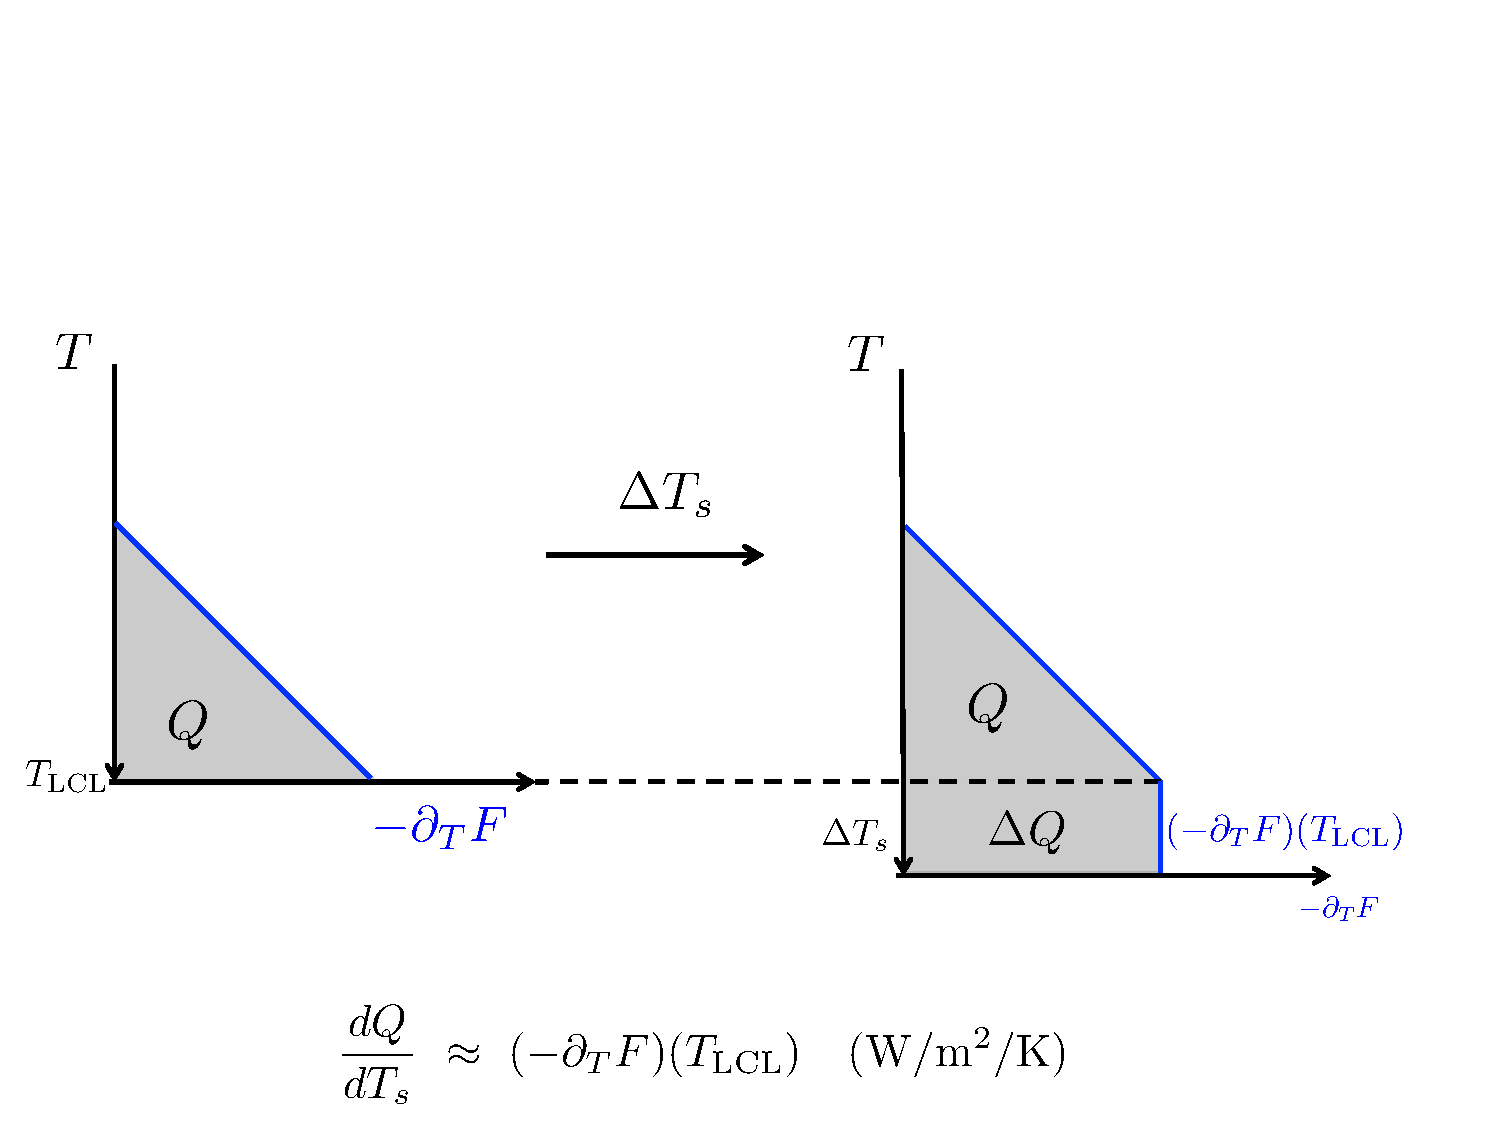
\includegraphics[scale=0.65,trim=0cm 0cm 0cm 5cm,clip=true]{../figures/dqdts_cartoon.pdf}
		\caption{Cartoon depicting the increase in $Q$ with \Ts\ in Eqn. \eqnref{dqdts}. Increasing the temperature range of the troposphere  exposes more of the \Ts-invariant curve $(\ppt F)(T)$ (blue lines). The contribution  of this newly exposed region to column-integrated cooling is given by Eqn. \eqnref{dqdts}.
		\label{dqdts_cartoon}
		}
	\end{center}
\end{figure}


%Figure Qnet_varsst
\begin{figure}[h]
	\begin{center}
			\includegraphics[scale=0.6]{../figures/Qnet_varsst.pdf}
		\caption{Column-integrated cooling $Q$ vs. \Ts\ (black circles), along with slopes $d Q/d \Ts$ (red lines) as diagnosed from \eqnref{dqdts}. These are shown for the SW (left), LW (center) and net (right) channels.  The black dashed lines connect the black circles and give a benchmark slope against which to compare the red lines. The `net' panel also gives CRM-diagnosed precipitation values in blue stars. Equation \eqnref{dqdts} does a good job of predicting $d Q/d \Ts$ for $\Ts < 310$ K. Above 310 K the qualitative agreement in the net and LW channel degrades, but \eqnref{dqdts} correctly predicts a leveling off of \QLW\ and \Qnet with increasing \Ts. 
		\label{Qnet_varsst}
		}
	\end{center}
\end{figure}

%Figure pptf_allchannels
\begin{figure}[h]
	\begin{center}
			\includegraphics[scale=0.6]{../figures/pptf_allchannels.pdf}
		\caption{As in Figs.  \ref{pptflw_tinv_dam} and \ref{pptfsw_tinv_dam}, but showing SW, LW, and net channels, including the \Ts=320 K simulation, and only using temperature coordinates. The LW cooling $-\ppt \FLW$ tends towards zero at high surface temperatures, causing the net cooling $-\ppt \Fnet$ to go negative. This drives the leveling off of  \Qnet and $P$ seen in Fig. \ref{Qnet_varsst}.
		\label{pptf_allchannels}
		}
	\end{center}
\end{figure}


%Figure wvp_check
\begin{figure}[h]
	\begin{center}
			\includegraphics[scale=0.8]{../figures/wvp_check.pdf}
		\caption{Comparison of \WVP\ as diagnosed from DAM (solid) to that estimated by \eqnref{WVP2} (dashed), in both linear and log coordinates.
		\label{wvp_check}
		}
	\end{center}
\end{figure}

 %Figure kappa_h2o
\begin{figure}[h]
        \begin{center}
                        \includegraphics[scale=1.75]{../figures/kappa_h2o.pdf}
                \caption{Minimum, maximum, median, and 25th and 75th percentile 
values of $\kappa$ for \htwo\ for 50 \cminverse\ intervals. Pulled from \cite{pierrehumbert2010}.
                \label{kappa_h2o}
                }
        \end{center}
\end{figure}




%%Figure sw_tinv
%\begin{figure}[h]
%	\begin{center}
%			\includegraphics[scale=0.6]{../figures/sw_tinv.pdf}
%		\caption{As in Fig. \ref{UD_tinv}, but for SW radiances \USW\ and \DSW, as well as flux \FSW.
%		\label{sw_tinv}
%		}
%	\end{center}
%\end{figure}
%
%%Figure ppzfnet_tinv
%\begin{figure}[h]
%	\begin{center}
%			\includegraphics[scale=0.8]{../figures/ppzfnet_tinv.pdf}
%		\caption{Shortwave, longwave, and net flux divergences as diagnosed from our various SST simulations. A rough \Ts-invariance is evident for $\ppz\FSW$ as for $\ppz \FLW$, but the spreads are opposite, yielding a $\ppz \Fnet$ profile that is strongly \Ts-invariant.
%		\label{ppzfnet_tinv}
%		}
%	\end{center}
%\end{figure}

\bibliographystyle{apa}
\bibliography{/Users/climateloaner/Dropbox/bibtex_mendeley/library}
%\bibliography{/Users/nadir/Dropbox/bibtex_mendeley/library}


\end{document}

